\section{Modelo conceptual}

La Figura~\ref{fig:conceptual} resume el dominio y ubica sus tres áreas. Las
figuras siguientes desarrollan cada área por separado para conservar las
cardinalidades sin concentrarlas en una sola lámina.

\begin{figure}[htbp]
\centering
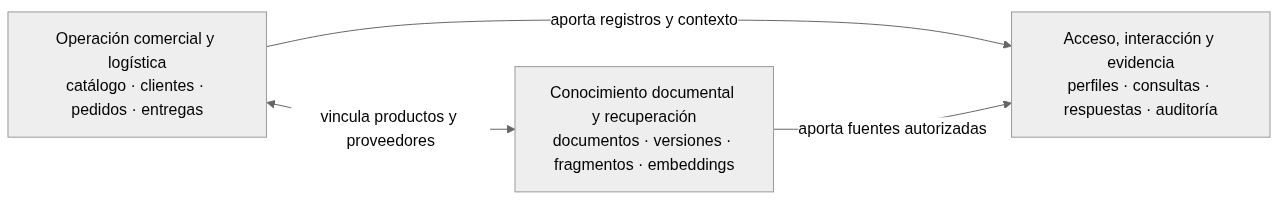
\includegraphics[width=0.9\textwidth]{modelo_conceptual.png}
\caption{Mapa conceptual general.}
\label{fig:conceptual}
\end{figure}
\FloatBarrier

\subsection{Operación comercial y logística}

\begin{landscape}
\begin{figure}[p]
\centering
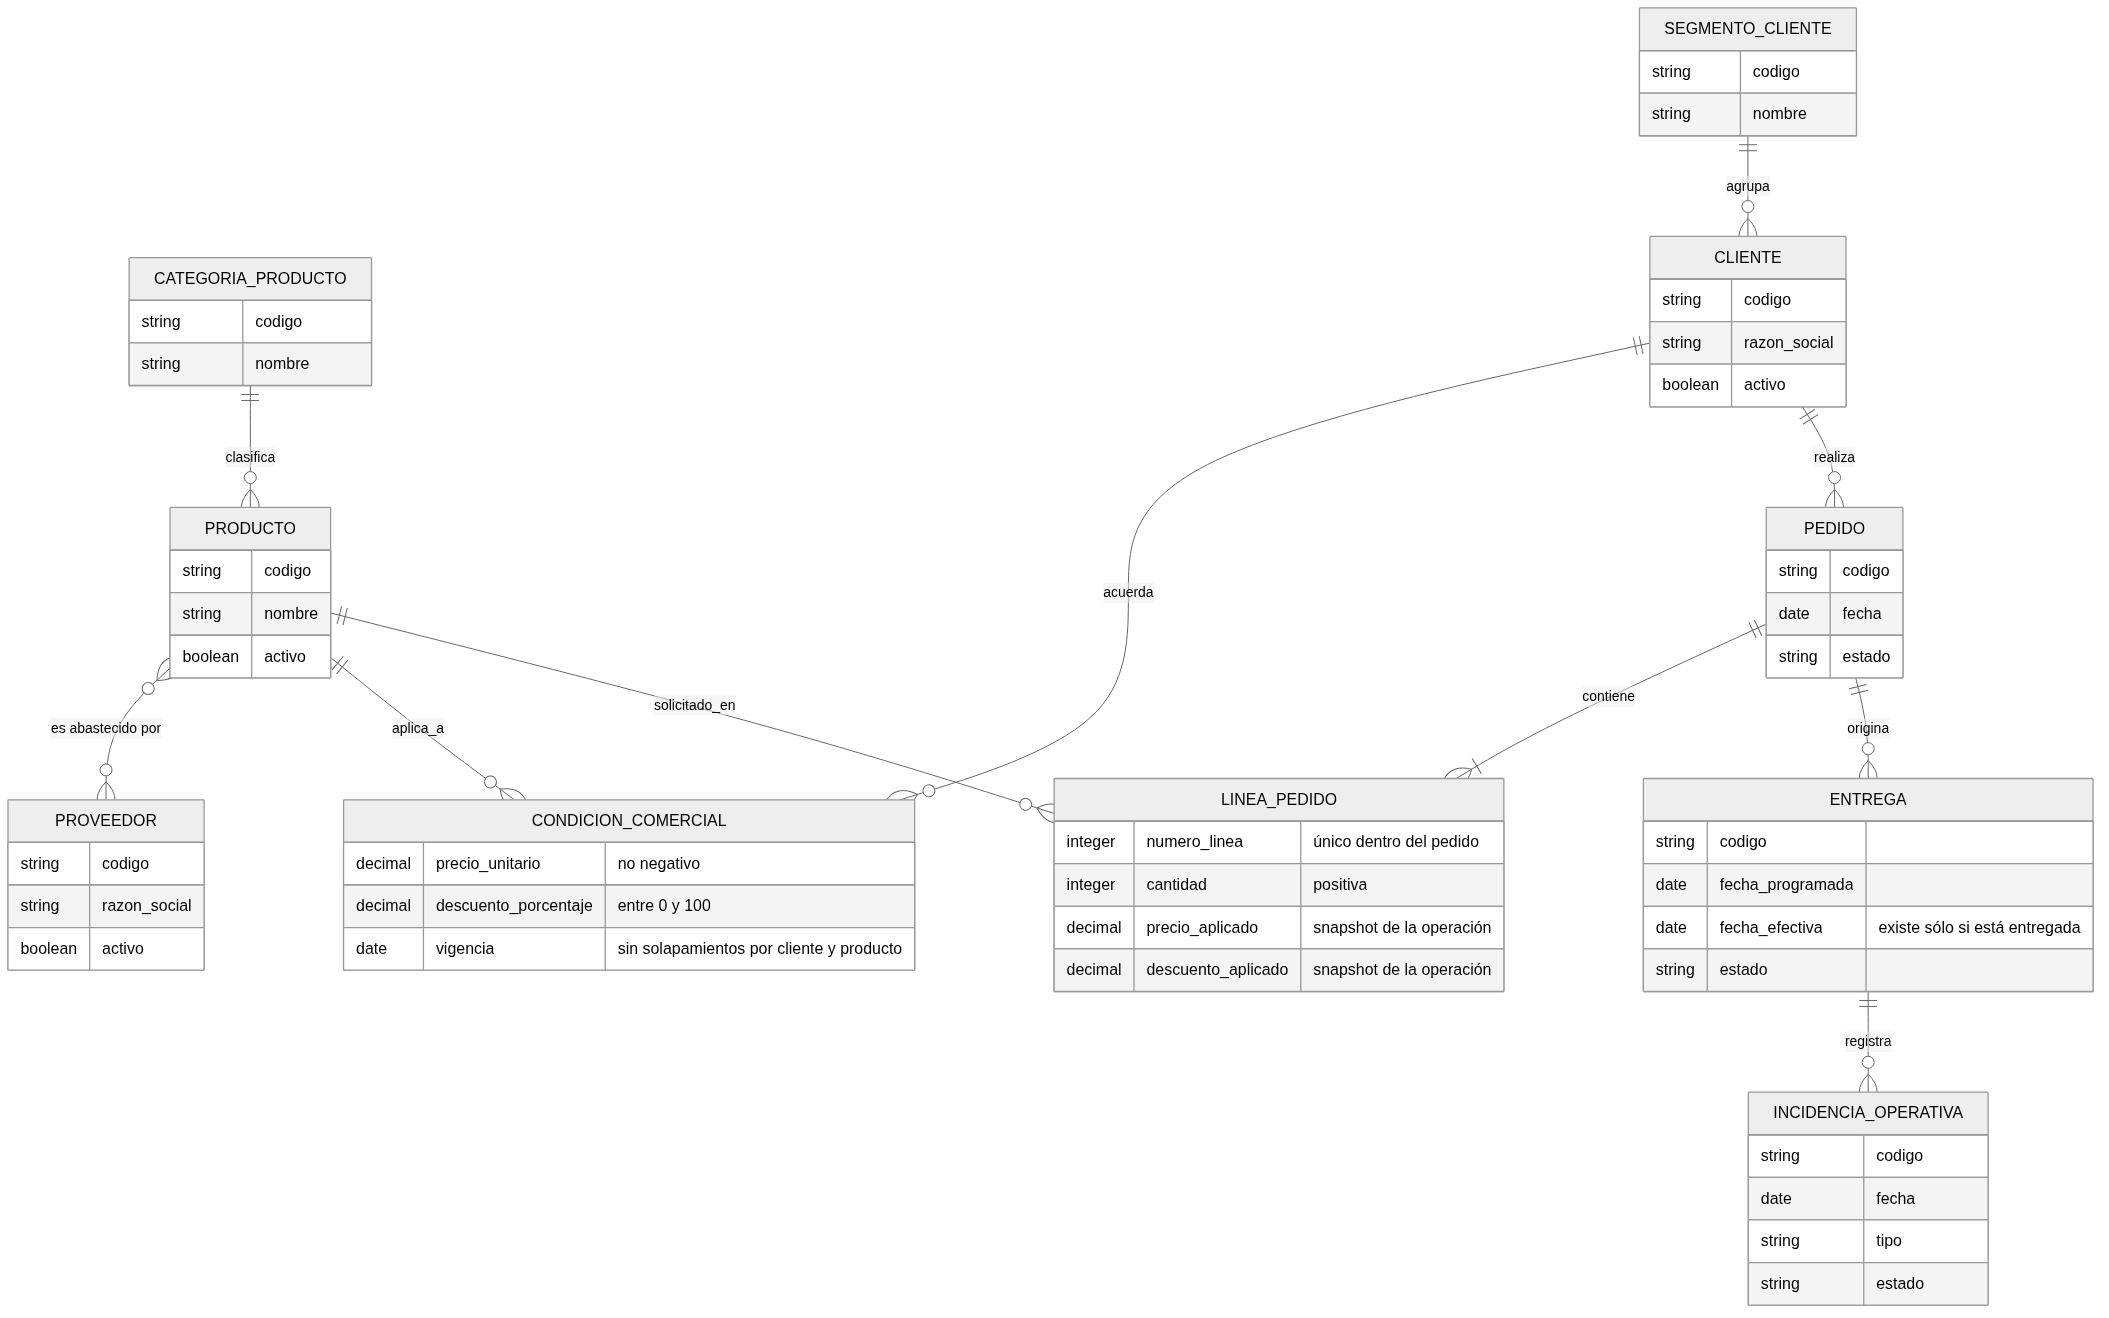
\includegraphics[width=0.85\linewidth]{conceptual_operacion.png}
\caption{Vista conceptual de la operación comercial y logística.}
\label{fig:conceptual-operacion}
\end{figure}
\end{landscape}

La Figura~\ref{fig:conceptual-operacion} relaciona clientes, productos,
condiciones comerciales, pedidos y entregas. Un pedido pertenece a un cliente
y contiene una o más líneas. Puede tener entregas parciales, y cada incidencia
se registra sobre una entrega. Las condiciones comerciales conservan su
vigencia; las líneas del pedido guardan el precio y el descuento aplicados en
el momento de la operación.
\FloatBarrier

\subsection{Documentos y recuperación}

\begin{figure}[htbp]
\centering
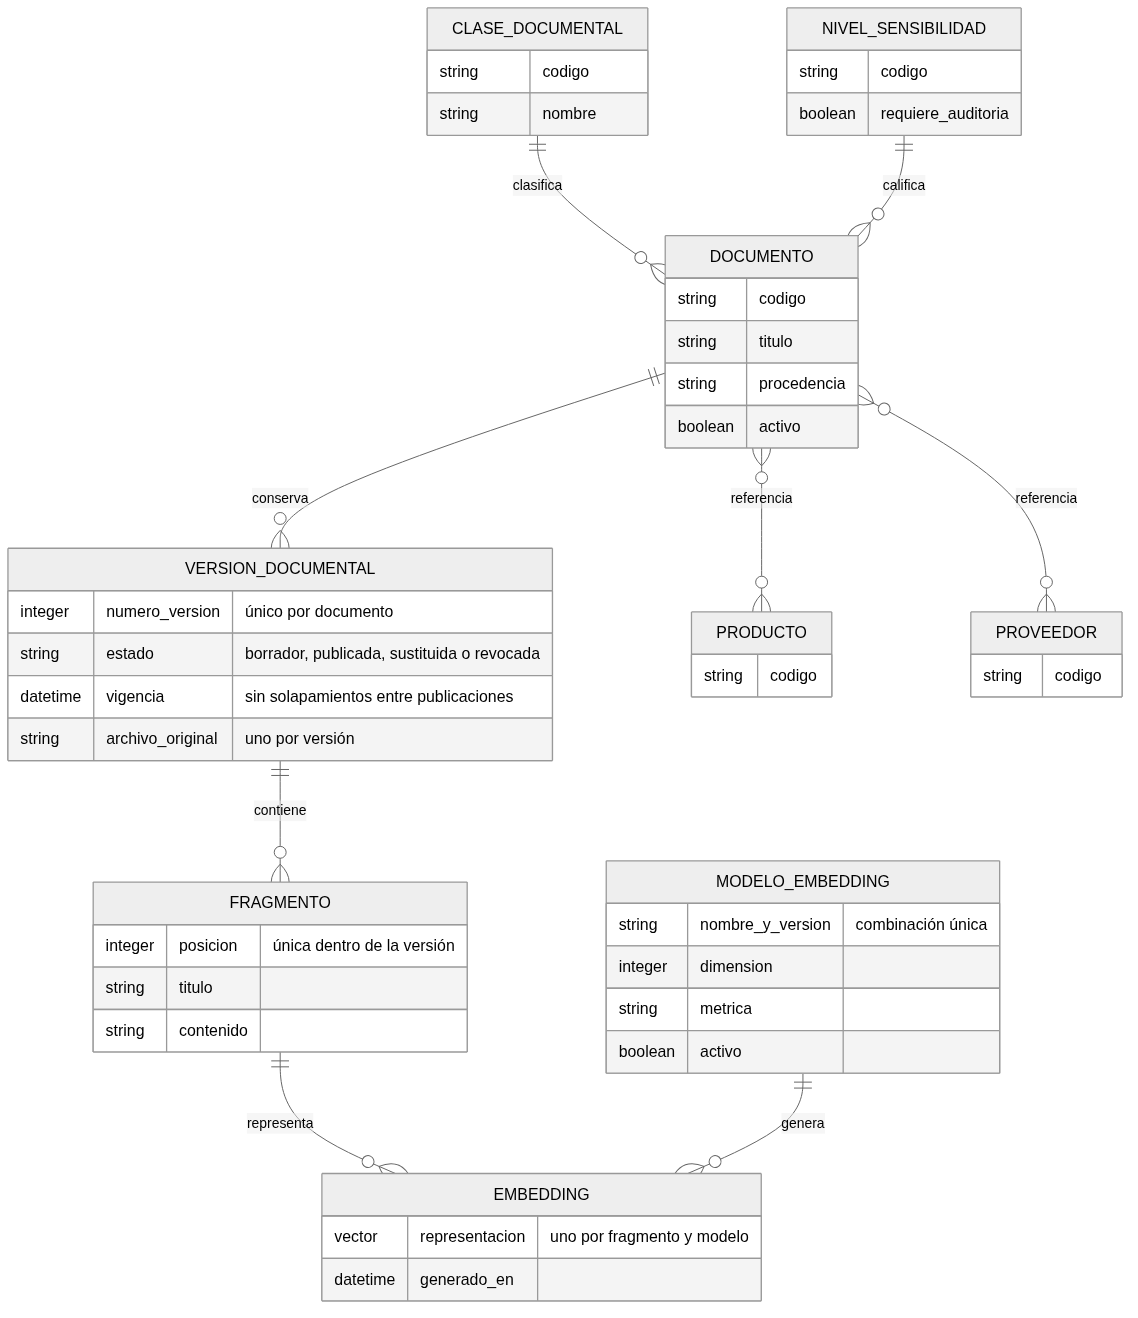
\includegraphics[width=\textwidth]{conceptual_documentos_recuperacion.png}
\caption{Vista conceptual de documentos y recuperación.}
\label{fig:conceptual-documentos}
\end{figure}

La Figura~\ref{fig:conceptual-documentos} muestra el recorrido desde un
documento hasta sus versiones, fragmentos y embeddings. Una versión puede
permanecer como borrador durante la carga. Sólo las versiones publicadas,
vigentes y autorizadas participan de la recuperación. Las versiones
sustituidas o revocadas se conservan para explicar respuestas anteriores.
\FloatBarrier

\subsection{Acceso, interacción y evidencia}

\begin{figure}[htbp]
\centering
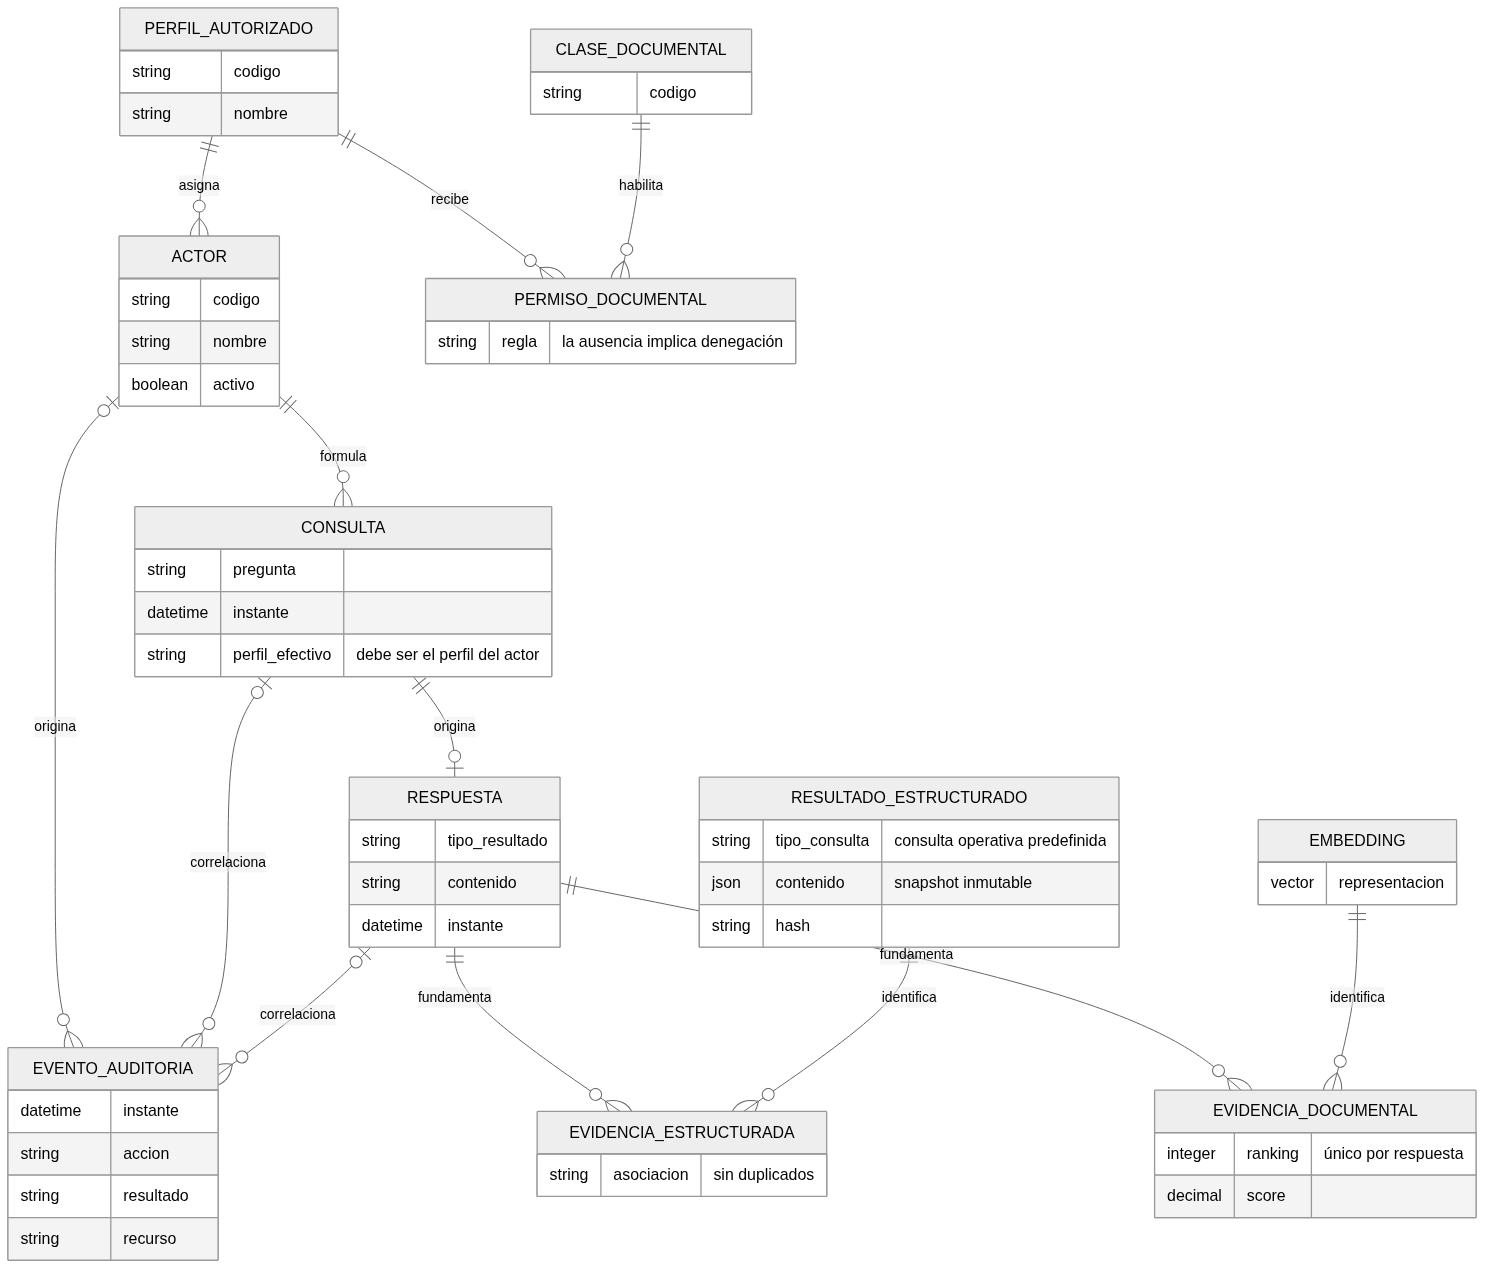
\includegraphics[width=\textwidth]{conceptual_acceso_interaccion_evidencia.png}
\caption{Vista conceptual de acceso, interacción y evidencia.}
\label{fig:conceptual-interaccion}
\end{figure}

La Figura~\ref{fig:conceptual-interaccion} vincula actores, perfiles, permisos,
consultas, respuestas y evidencia. Cada actor tiene un perfil autorizado y el
permiso se define por clase documental. Una respuesta exitosa debe conservar
evidencia documental o estructurada; los resultados negativos no admiten
evidencia. Los eventos de auditoría registran el actor, el perfil efectivo y
la correlación necesaria para reconstruir la interacción.
\FloatBarrier
